De acuerdo con \cite{IR-book} Recuperación de Información o IR por sus siglas en inglés hace referencia a la encontrar material que satisfaga una necesidad de información. Usualmente, este material son documentos de texto y se almacena en computadores. Hasta hace algunos años esta actividad se limitaba a algunas profesiones específicas. No obstante, el \textit{boom} del internet ha ocasionado que la mayoría de estas búsquedas se hagan a través de este, sea mediante motores de búsqueda o correo electrónico.\\

Para IR se han propuesto diferentes métodos que permiten solucionar el problema desde diferentes ángulos.

\textbf{TODO}
\begin{itemize}
    \item Focus más a NLP.
    \item Hablar del dataset.
    \item Hablar de la importancia de IR.
\end{itemize}

\subsection*{Preprocesamiento}

Antes de implementar las distintas estrategias de recuperación de información, se realizo un preprocesamiento igual a todo el \textit{dataset}. Con este proceso se busca representar tanto los \textit{queries} como los documentos de forma numérica de manera tal que dicha representación ayude a resolver el problema de IR. Para esto se le aplicaron distintos procesamientos estándar, los cuales se presentan de forma resumida en la figura \ref{fig:preprocess}. Todo el código correspondiente a esta sección se encuentra en el cuaderno \texttt{HW01\_Utilities.ipynb}.

\begin{figure}[H]
    \centering
    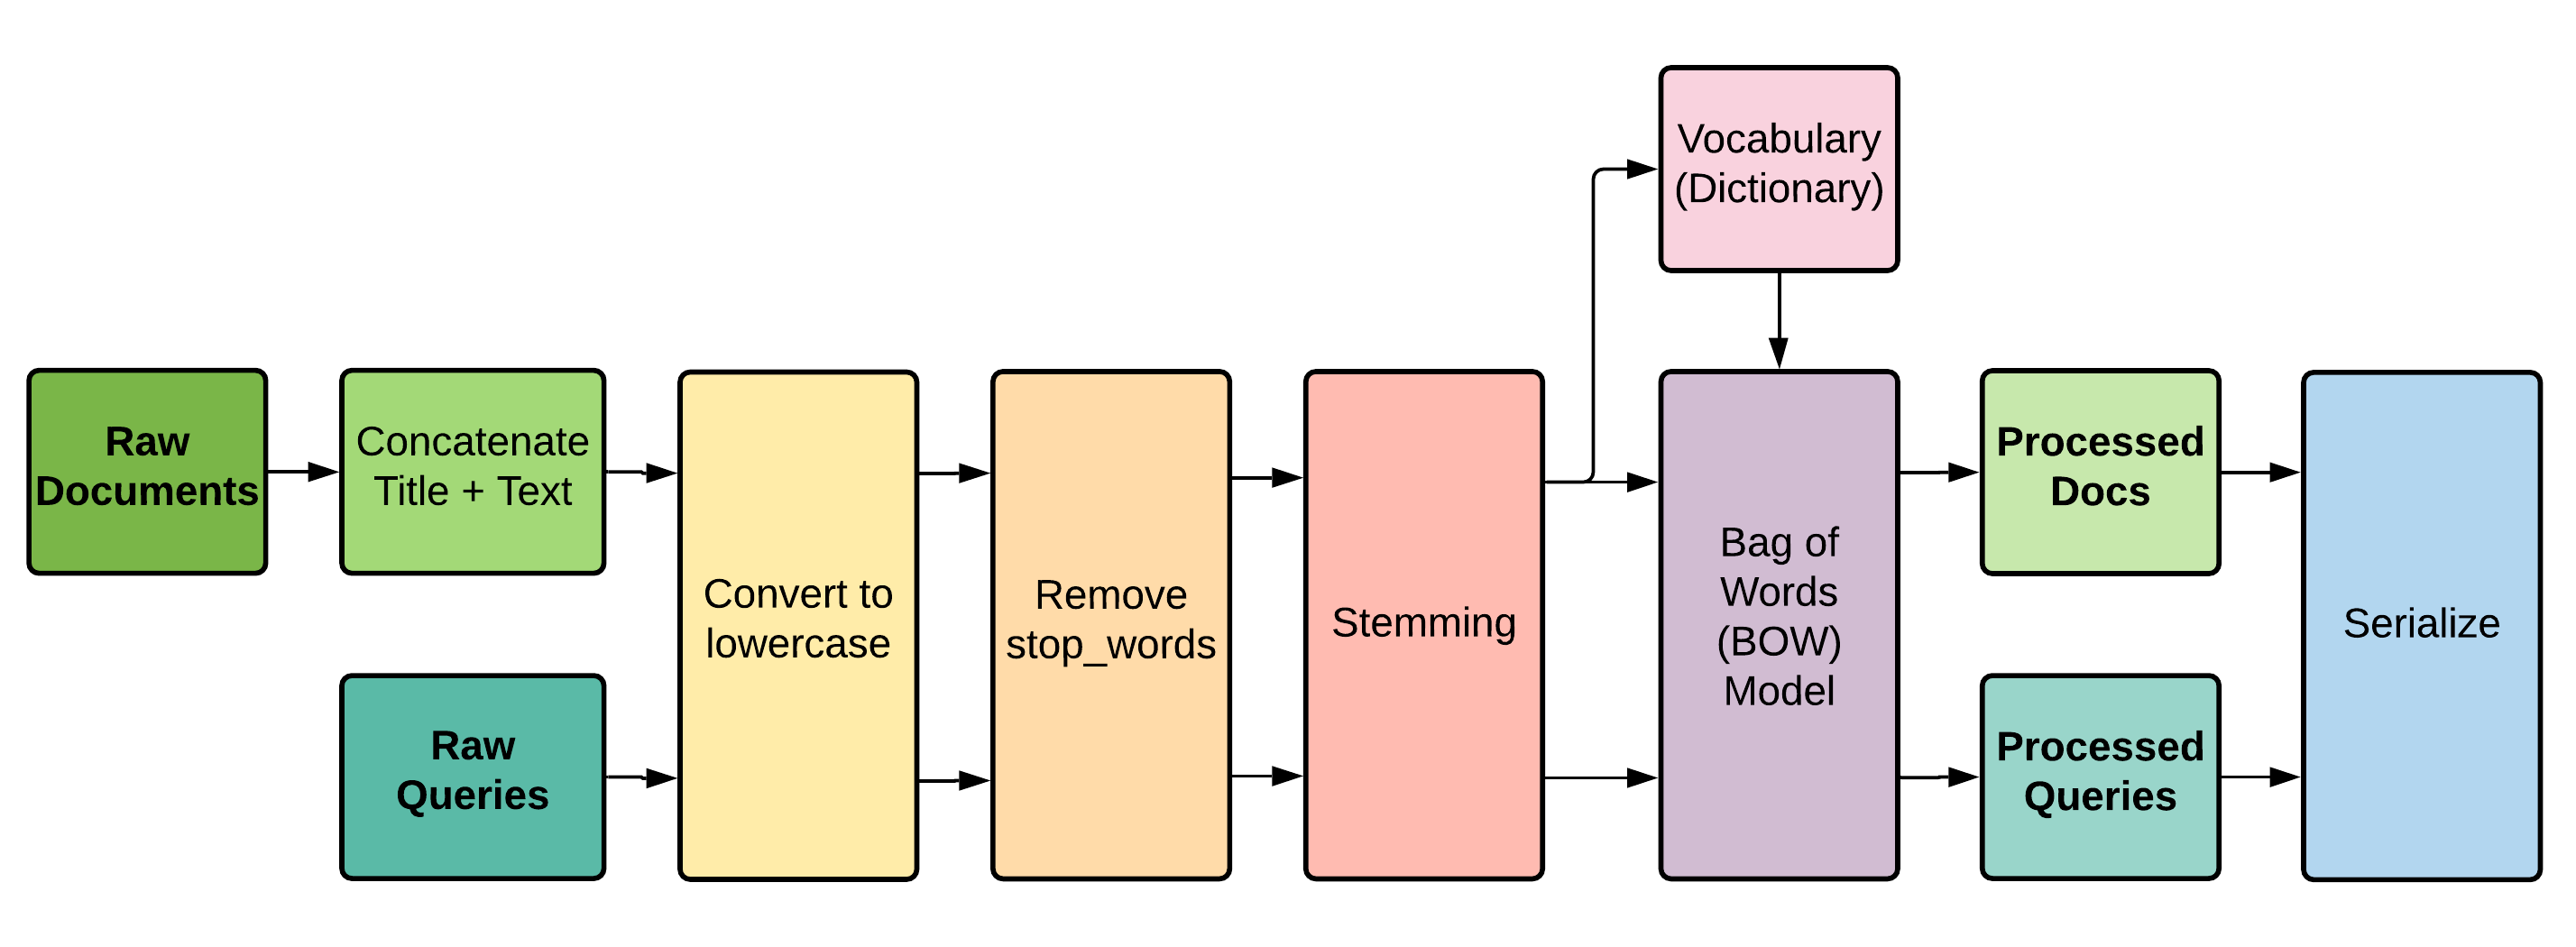
\includegraphics[width=0.95\textwidth]{doc/images/preprocesamiento.png}
    \caption{Etapas de procesamiento aplicadas al texto para resolver el problema de IR}
    \label{fig:preprocess}
\end{figure}

A grande rasgos lo que se hace es tomar el texto crudo (para los documentos se concatena el titulo con su cuerpo) y se convierten todos los caracteres a minúscula. Posteriormente, se remueven las \textit{stop words} (palabras comunes para el idioma inglés) y se reducen todas las palabras a su raíz con \textit{stemming}, todo esto con la librería \texttt{gensim.parsing} y las funciones de \texttt{remove\_stopwords} y \texttt{PorterStemer}, respectivamente. Vale la pena aclarar, que el proceso de \textit{stemming} no reduce las palabras a su raíz semántica sino con una serie de reglas establecidas para el idioma. Finalmente, con los términos (únicamente de el corpus de documentos) se construye el vocabulario (o \textit{dictionary}) y a partir de este los modelos de Bag of words (BOW), tanto para los documentos como para los \textit{queries}. Por último, estos se serializan para poder utilizarse en los distintos cuadernos donde se implementan las distintas estrategias de recuperación de información.